\section{Analysis techniques}
\label{sec:method} 
We address imaging systematics in DESI data by performing a separate treatment for each imaging region (e.g., DECaLS North) within the DESI footprint to reduce the impact of systematic effects specific to that region. Once the imaging systematic weights are obtained for each imaging region separately, we combine the data from all regions to compute the power spectrum for the entire DESI footprint to increase the overall statistical power and enable more robust measurements of $\fnl$. We then conduct robustness tests on the combined data to assess the significance of any remaining systematic effects.


\subsection{Power spectrum estimator}
We first construct the density contrast field from the LRG density, $\rho$,
\begin{align}\label{eq:delta}
    \delta_{g} &= \frac{\rho- \overline{\rho}}{\overline{\rho}},
\end{align}
where the mean galaxy density $\overline{\rho}$ is estimated from the entire LRG sample. As a robustness test, we also analyze the power spectrum from each imaging region individually, in which $\overline{\rho}$ is calculated separately for each region. Then, we use the pseudo angular power spectrum estimator \citep{hivon2002master},
\begin{equation}\label{eq:pusedocell}
        \tilde{C}_{\ell} = \frac{1}{2\ell +1} \sum_{m=-\ell}^{\ell} |a_{\ell m}|^{2},
\end{equation}
where the coefficients $a_{\ell m}$ are obtained by decomposing $\delta_{g}$ into spherical harmonics, $Y_{\ell m}$,
\begin{equation}\label{eq:alm}
        a_{\ell m} = \int d\Omega ~ \delta_{g} W Y^{*}_{\ell m},
\end{equation}
where $W$ represents the survey window that is described by the number of randoms normalized to the expected value.

We use the implementation of \texttt{anafast} from the \textsc{HEALPix} package \citep{gorski2005healpix} to do fast harmonic transforms (Equation \ref{eq:alm}) and estimate the pseudo angular power spectrum of the LRG targets and the cross power spectrum between the LRG targets and the imaging systematic maps.

\subsection{Modelling}
The estimator in Equation \ref{eq:pusedocell} yields a biased power spectrum when the survey sky coverage is incomplete. Specifically, the survey mask causes correlations between different harmonic modes \citep{beutler2014clustering,wilson2017rapid}, and the measured clustering power is smoothed on scales near the survey size. An additional potential cause of systematic error arises from the fact that the mean galaxy density used to construct the density contrast field (Equation \ref{eq:delta}) is estimated from the available data, rather than being known a priori. This introduces what is known as an integral constraint effect, which can cause the power spectrum on modes near the size of the survey to be artificially suppressed, effectively pushing it towards zero \citep{peacock1991large,de2019integral}. Since $\fnl$ is highly sensitive to the clustering power on these scales, it is crucial to account for these systematic effects in the model galaxy power spectrum to obtain unbiased $\fnl$ constraints \citep[see, also,][]{riquelme2022primordial}, which we describe below.
  
The other theoretical systematic issues are however subdominant in the angular power spectrum. For instance, relativistic effects generate PNG-like scale-dependent signatures on large scales, which interfere with measuring $\fnl$ with the scale-dependent bias effect using higher order multipoles of the 3D power spectrum \citep{wang2020}. Similarly, matter density fluctuations with wavelengths larger than survey size, known as super-sample modes, modulate the galaxy 3D power spectrum \citep{castorina2020JCAP}. In a similar way, the peculiar motion of the observer can mimic a PNG-like scale-dependent signature through aberration, magnification and the Kaiser-Rocket effect, i.e., a systematic dipolar apparent blue-shifting in the direction of the observer's peculiar motion \citep{2021JCAP...11..027B}.
  
\subsubsection{Angular power spectrum} 
The relationship between the linear matter power spectrum $P(k)$ and the projected angular power spectrum of galaxies is expressed by the following equation:
\begin{equation}\label{eq:cell}
C_{\ell} = \frac{2}{\pi}\int_{0}^{\infty}\frac{dk}{k}k^{3}P(k)|\Delta_{\ell}(k)|^{2} + N_{\rm shot},
\end{equation}
where $N_{\rm shot}$ is a scale-independent shot noise term. The projection kernel $\Delta_{\ell}(k) = \Delta^{\rm g}_{\ell}(k) + \Delta^{\rm RSD}_{\ell}(k) + \Delta^{\mu}_{\ell}(k)$ includes redshift space distortions \mr{and magnification bias,} and determines the contribution of each wavenumber $k$ to the galaxy power spectrum on mode $\ell$. For more details on this estimator, refer to \cite{Padmanabhan2007}. The non-linearities in the matter power spectrum are negligible for the scales of interest \citep[see, e.g.,][]{Ho2015JCAP...05..040H}. For $\ell=40$, $\Delta_{\ell}(k)$ peaks at $k\sim 0.02~ h\text{Mpc}^{-1}$, which is above the non-linear regime. The FFTLog\footnote{\href{https://github.com/xfangcosmo/FFTLog-and-beyond}{github.com/xfangcosmo/FFTLog-and-beyond}} algorithm and its extension as implemented in \cite{fang2020beyond} are employed to calculate the integrals for the projection kernel $\Delta_{\ell}(k)$, which includes the $l^{\rm th}$ order spherical Bessel functions, $ j_{\ell}(kr)$, and its second derivatives,
\begin{align}
    \Delta^{\rm g}_{\ell}(k) &= \int \frac{dr}{r} r (b+\Delta b) D(r) \frac{dN}{dr} j_{\ell}(kr),\\
    \Delta^{\rm RSD}_{\ell}(k) &= - \int \frac{dr}{r} r f(r) D(r) \frac{dN}{dr} j^{\prime\prime}_{\ell}(kr),\\
    \Delta^{\mu}_{\ell}(k) &= - \ell(\ell+1) \int dr D(r) W_{\mu}(z) j_{\ell}(kr),
\end{align}
where $b$ is the linear bias (dashed curve in Figure \ref{fig:nz}), $D$ represents the linear growth factor normalized as $D(z=0)=1$, $f(r)$ is the growth rate, and $dN/dr$ is the redshift distribution of galaxies normalized to unity and described in terms of comoving distance\footnote{$dN/dr = (dN/dz)(dz/dr) \propto (dN/dz)H(z)$} (solid curve in Figure \ref{fig:nz}). \mr{The magnification bias window function $W_{\mu}(z)$ is}
\begin{equation}
W_{\mu}(z) = (5s-2)\frac{3H^{2}_{0}\Omega_{m}(1+z)}{2c^{2}k^{2}} \int_{z}^{\infty} dz^{\prime}\frac{dN}{dz} \frac{r(z^{\prime}) - r(z)}{r(z^{\prime})r(z)},
\end{equation}
\mr{where $\Omega_{m}$ is the matter density, $H_{0}$ is the Hubble constant\footnote{$H_{0}=100~({\rm km}~{\rm s}^{-1})/(h^{-1}{\rm Mpc})$ and $k$ is in unit of $h {\rm Mpc}^{-1}$}, $c$ is the speed of light, and $s$ is the slope of the number count function \citep{2008PhRvD..77b3512L} which quantifies the response of the number density of galaxies to achromatic changes in the brightness. The parameter $s$ is estimated by shifting all magnitudes by an infinitesimal amount and re-running the color-mag selection, with the caveat that for a fiber flux-selected sample, like the DESI LRG targets, the impact of magnification on fiber flux depends on the shape parameters for each morphology type \citep{zhou2023desi}. The parameter $s$ for our sample is found to vary slightly in the different imaging regions: $s=0.951\pm 0.011$ for BASS+MzLS, $s=0.943 \pm 0.007$ for DECaLS North+DECaLS South, and $s=0.945\pm 0.006$ for DESI\footnote{Private communication with Dr. Rongpu Zhou.}. We fix $s$ to the central values in our analysis.} The PNG-induced scale-dependent shift is given by \citep{slosar2008constraints}
\begin{equation}
\Delta b = b_{\phi}(z) \fnl \frac{3 \Omega_{m} H^{2}_{0}}{2 k^{2}T(k)D(z) c^{2}} \frac{g(\infty)}{g(0)},
\label{eq:scaledepbias}
\end{equation}
where $T(k)$ is the transfer function, and $g(\infty)/g(0) \sim 1.3$ with $g(z)\equiv (1+z) D(z)$ is the growth suppression due to non-zero $\Lambda$ because of our normalization of $D$ \citep[see, e.g.,][]{2010JCAP...07..013R, 2019MNRAS.485.4160M}. We assume the universality relation which directly relates $b_\phi$ to $b$ via $b_{\phi} = 2 \delta_{c}(b - p)$ with $\delta_{c}= 1.686$ representing the critical density for spherical collapse \citep{fillmore1984self}. We fix $p=1$ in our analysis and marginalize over b \citep[see, also,][]{slosar2008constraints,2010JCAP...07..013R,2013MNRAS.428.1116R}. 

\begin{figure}
\centering
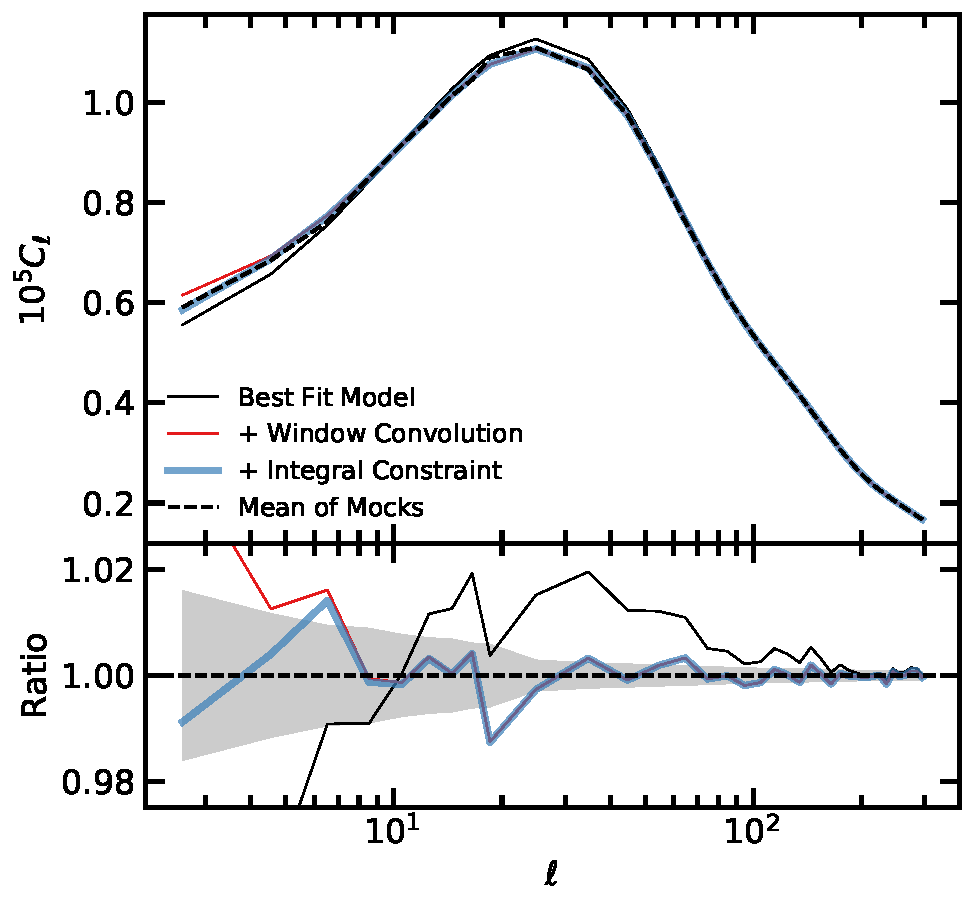
\includegraphics[width=0.45\textwidth]{model_mock.pdf}
\caption{The mean power spectrum from the $\fnl=0$ mocks (no contamination) and best-fitting theoretical prediction after accounting for the survey geometry and integral constraint effects. Bottom panel shows the residual power spectrum relative to the mean power spectrum. The dark and light shades represent the $68\%$ error on the mean and one realization, respectively. No imaging systematic cleaning is applied to these mocks.}\label{fig:model_mock}
\end{figure}

\subsubsection{Survey geometry and integral constraint}
We employ a technique similar to the one proposed by \cite{chon2004fast} to account for the impact of the survey geometry on the theoretical power spectrum. The ensemble average for the partial sky power spectrum is related to that of the full sky power spectrum via a mode-mode coupling matrix, ${\rm M}_{\ell \ell^{\prime}}$,
\begin{equation}\label{eq:mixm}
    <\tilde{C}_{\ell}> = \sum_{\ell^{\prime}} {\rm M}_{\ell \ell^{\prime}}<C_{\ell^{\prime}}>.
\end{equation}
We convert this convolution in the spherical harmonic space into a multiplication in the correlation function space. Specifically, we first transform the theory power spectrum (Equation \ref{eq:cell}) to the correlation function, $\hat{\omega}^{\rm model}$. Then, we estimate the survey mask correlation function, $\hat{\omega}^{\rm window}$, and obtain the pseudo-power spectrum,
\begin{align}
    \tilde{C}^{\rm model}_{\ell} &= 2\pi \int \hat{\omega}^{\rm model}\hat{\omega}^{\rm window}~P_{\ell}(\cos\theta) d\cos\theta.
\end{align}
\mr{Figure \ref{fig:mask2pf} illustrates ${\hat \omega}^{\rm window}$ for the different masks representing the DESI footprint and its imaging sub-regions. We present a benchmark of our method against the direct mode-mode coupling matrix approach in Appendix \ref{ssec:windowconv}.} 

The integral constraint is another systematic effect which is induced since the mean galaxy density is estimated from the observed galaxy density, and therefore is biased by the limited sky coverage \citep{peacock1991large}. To account for the integral constraint, the survey mask power spectrum is used to introduce a scale-dependent correction factor that needs to be subtracted from the power spectrum as,
\begin{equation}
     \tilde{C}^{\rm model, IC}_{\ell} = \tilde{C}^{\rm model}_{\ell} - \tilde{C}^{\rm model}_{\ell=0} \left(\frac{\tilde{C}^{\rm window}_{\ell}}{\tilde{C}^{\rm window}_{\ell=0}}\right),
\end{equation}
where $\tilde{C}^{\rm window}$ is the survey mask power spectrum, i.e., the spherical harmonic transform of $\hat{\omega}^{\rm window}$.

\begin{figure}
    \centering
    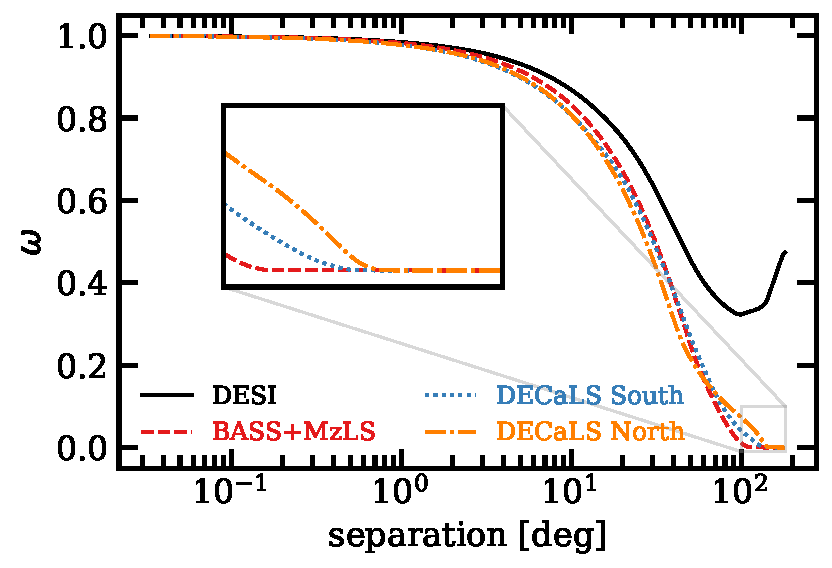
\includegraphics[width=0.45\textwidth]{figures/mask_2pf.pdf}
    \caption{\mr{The survey mask correlation functions for the imaging regions forming the DESI footprint as a function of angular separation. The inset shows the correlations specifically for angles between $100$ and $180$ degrees.}}
    \label{fig:mask2pf}
\end{figure}



The lognormal simulations are used to validate our survey window and integral constraint correction. Figure \ref{fig:model_mock} shows the mean power spectrum of the $\fnl=0$ simulations (dashed) and the best-fitting theory prediction before and after accounting for the survey mask and integral constraint. The simulations are neither contaminated nor mitigated. The light and dark shades represent the 68\% estimated error on the mean and one single realization, respectively. The DESI mask, which covers around $40\%$ of the sky, is applied to the simulations. We find that the survey window effect modulates the clustering power on $\ell < 200$ and the integral constraint alters the clustering power on $\ell < 6$.

\subsection{Parameter estimation}

\begin{figure*}
\centering
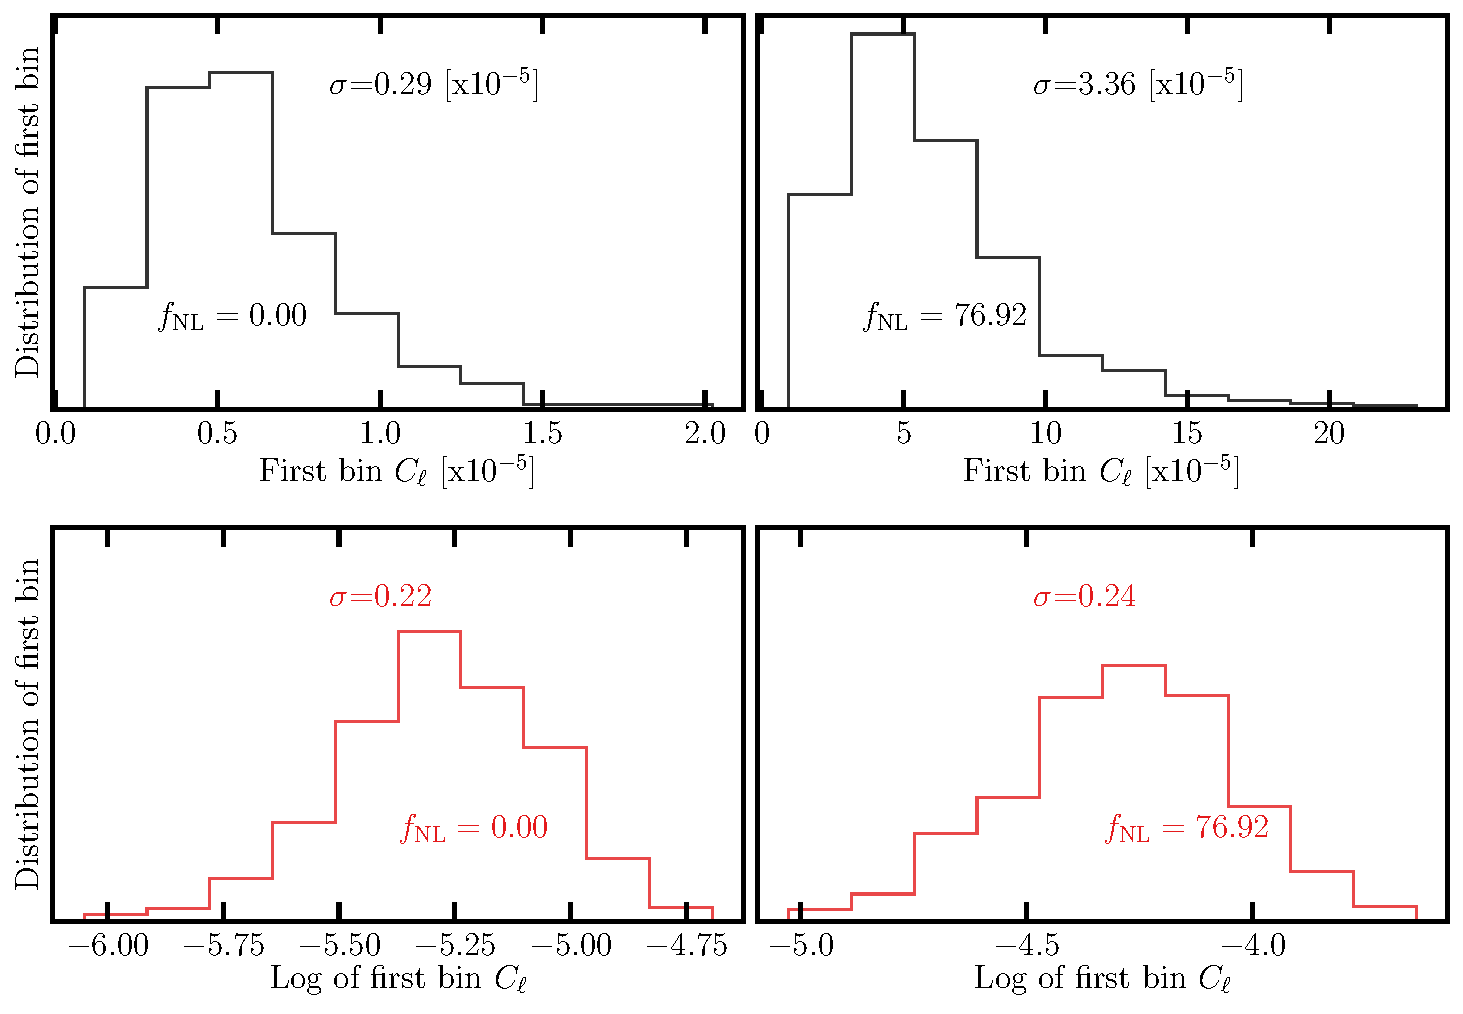
\includegraphics[width=0.85\textwidth]{hist_cl.pdf}
\caption{The distribution of the first bin power spectra and its log transformation from the simulations with $\fnl=0$ (left) and $76.9$ (right). The log transformation largely removes the asymmetry in the distributions.}\label{fig:histcell}
\end{figure*}

Our parameter inference uses standard MCMC sampling. A constant clustering amplitude is assumed to determine the redshift evolution of the linear bias of our DESI LRG targets, $b(z) = b/D(z)$, which is supported by the HOD fits to the angular power spectrum \citep{zhou2021clustering}. In MCMC, we allow $\fnl$, $N_{\rm shot}$, and $b$ to vary, while all other cosmological parameters are fixed at the fiducial values (see \S \ref{ssec:mocks}). The galaxy power spectrum is divided into a discrete set of bandpower bins with $\Delta\ell=2$ between $\ell=2$ and $20$ and $\Delta \ell=10$ from $\ell=20$ to $300$. Each clustering mode is weighted by $2\ell+1$ when averaging over the modes in each bin.

The expected large-scale power is highly sensitive to the value of $\fnl$ such that the the amplitude of the covariance for $C_{\ell}$ is influenced by the true value of $\fnl$, see also \cite{2013MNRAS.428.1116R} for a discussion. As illustrated in the top row of Figure \ref{fig:histcell}, we find that the distribution of the power spectrum at the lowest bin, $2\leq \ell < 4$, is highly asymmetric and its standard deviation varies significantly from the simulations with $\fnl=0$ to $76.9$. We can make the covariance matrix less sensitive to $\fnl$ by taking the log transformation of the power spectrum, $\log C_{\ell}$. As shown in the bottom panels in Figure \ref{fig:histcell}, the log transformation reduces the asymmetry and the difference in the standard deviations between the $\fnl=0$ and $76.9$ simulations. Therefore, we minimize the negative log likelihood defined as,
\begin{equation}\label{eq:likelihood}
-2\log \mathcal{L} = (\log \tilde{C}(\Theta)-\log \tilde{C})^{\dagger} \mathbb{C}^{-1} (\log \tilde{C}(\Theta)-\log \tilde{C}),
\end{equation}
where $\Theta$ represents a container for the parameters $\fnl$, $b$, and $N_{\rm shot}$; $\tilde{C}(\Theta)$ is the (binned) expected pseudo-power spectrum; $\tilde{C}$ is the (binned) measured pseudo-power spectrum; and $\mathbb{C}$ is the covariance on $\log\tilde{C}$ constructed from the $\fnl=0$ log-normal simulations. Log-normal simulations have been commonly used and validated to estimate the covariance matrices for galaxy density fields, and non-linear effects are subdominant on the scales of interest to $\fnl$ \citep[see, e.g.,][]{2017MNRAS.466.1444C, 2021MNRAS.508.3125F}. We also test for the robustness of our results against an alternative covariance constructed from the $\fnl=76.9$ mocks. Flat priors are implemented for all parameters: $\fnl \in [-1000, 1000]$, $N_{\rm shot} \in [-0.001, 0.001]$, and $b \in [0, 5]$. 


\subsection{Calibration of over-correction}\label{ssec:calibration}

The template-based mitigation of imaging systematics removes some of the true clustering signal, and \mout{the amount of the removed signal increases as more maps are used for the regression.} \mr{mitigating with more maps should remove more modes and thus both bias the $\fnl$ estimation and the uncertainty.} We calibrate the over-correction effect using the mocks presented in \S \ref{sec:data}. \mr{One of the main advantages of having two sets of mocks with low and high power at low $\ell$ is that it gives a model for mapping the whole posterior and thus learning how the $\fnl$ constraints degrade as the imaging systematic correction gets greater.}  We apply the neural network model to both the $\fnl=0$ and $76.9$ simulations, with and without imaging systematics, using various sets of imaging systematic maps. Specifically, we consider \textit{non-linear three maps}, \textit{non-linear four maps}, and \textit{non-linear nine maps}. Then, we measure the power spectra from the mocks. We fit both the mean power spectrum and each individual power spectrum from the mocks. \mr{Appendix \ref{ssec:contmocks} presents the impact of the non-linear methods on the mock power spectra, and here we summarize the relevant details for the calibration of over-correction.}

Figure \ref{fig:fnlbias} displays a comparison between the estimates of $\fnl$ before and after mitigation for the clean mocks. The best-fitting estimates \mr{from the mean of the mocks} are represented by the solid curves, and the individual spectra results are displayed as the scatter points. The results from fitting the mean power spectrum of the contaminated mocks are also shown via the dashed curves. We find nearly identical results for the biases caused by mitigation, whether or not the mocks have any contamination, which can be seen by observing the solid and dashed curves displayed on Figure \ref{fig:fnlbias} (see, also, Figure \ref{fig:clmocks}, for a comparison of the mean power spectrum). For clarity, the best-fitting estimates for the individual contaminated data are not shown in the figure.

\begin{figure}
\centering
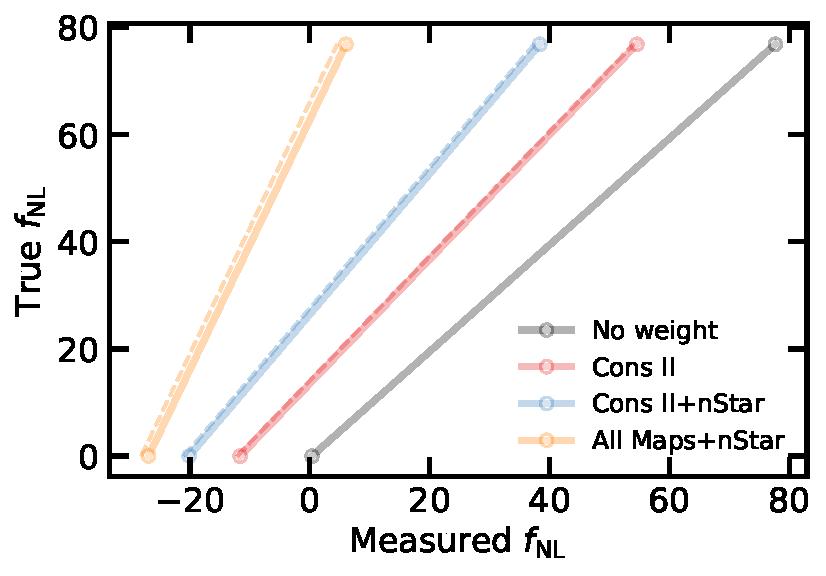
\includegraphics[width=0.45\textwidth]{figures/fnlbias}
\caption{The \textit{No mitigated, clean} vs \textit{mitigated} $\fnl$ values from the $\fnl=0$ and $76.9$ mocks. The solid (dashed) lines represent the best-fitting estimates from fitting the mean power spectrum of the clean (contaminated) mocks. The scatter points show the best-fitting estimates from fitting the individual spectra for the clean mocks.}\label{fig:fnlbias}
\end{figure}


\mr{As summarized in Table \ref{tab:contmocksmcmc}, we find significant shifts in the best-fitting estimates of $\fnl$ from the fits to the mean spectra. Specifically, we obtain $\Delta \fnl=-12$ for non-linear three maps, $-20$ for non-linear three maps, and $-27$ for non-linear nine maps when analyzing the $\fnl=0$ mocks. Whereas, bigger shifts are noticed for $\fnl=76.9$: we find $\Delta \fnl=-23$ for non-linear three maps, $-39$ for non-linear four maps, and $-72$ for non-linear nine maps.}

To calibrate our methods, we fit a linear curve to the $\fnl$ estimates from the mean power spectrum of the mocks, $f_{\rm NL, no~mitigation, clean} = m_{1} f_{\rm NL, mitigated} + m_{2}$. The $m_{1}$ and $m_{2}$ coefficients for non-linear three, four, and nine maps are summarized in Table \ref{tab:debiasparams}. These coefficients represent the impact of the cleaning methods on the likelihood. The uncertainty in $\fnl$ after mitigation increases by $m_{1}-1$. Figure \ref{fig:fnlbias} also shows that the choice of our cleaning method can have significant implications for the accuracy of the measured $\fnl$, and careful consideration should be given to the selection of the primary imaging systematic maps and the calibration of the cleaning algorithms in order to minimize systematic uncertainties.


\begin{table}
\begin{center}
\caption{Linear parameters employed to de-bias the $\fnl$ constraints to account for the over-correction issue.}\label{tab:debiasparams}
\begin{tabular}{lcc}
\hline
\hline
\textbf{Cleaning Method} & $m_{1}$ & $m_{2}$ \\
\hline
Nonlinear Three Maps & 1.17 & 13.95 \\
Nonlinear Four Maps & 1.32 & 26.97 \\
Nonlinear Nine Maps & 2.35 & 63.5\\
\hline
\end{tabular}
\end{center}
\end{table}
